\normallinespacing

\chapter{Introduction}
\section{Problem Statement}

Difficulty factors in games are rarely discussed as important. In some games, they are well-thought-out additions, built for the hardcore players. Taking into account that the difficulty of a game is centered on the player and reflects his or her skills, these skills, therefore, change depending on the type of game or the condition of the player. For example: the skills used by a player who is used to playing shooting games may not be suitable for platforming games. Consequently, their score in a platforming game would also be lower considering that different reflexes and motor skills are needed. These are, of course, quite large suppositions, on which we will rest the main question belying our hypothesis: What are the factors that affect the difficulty of video games for humans?

In this work, we will analyze the importance of different types of difficulty in video games to better understand what are the components that make video games hard or easy for humans. We chose video games as the task because many researchers are focused on solving video games but only a few of them are focused on humans. \cite{Dubey2018HumanPriors}

\section{State of the Art}
Why are humans so good at solving complex video games? Which factors determine whether a video game is hard or easy for humans? We will try to address these questions and others as part of this research project. The idea is to go deeper into the difficulty of video games and their main components.  \cite{Dubey2018HumanPriors}

We start from Juul’s definition to explain why difficulty scaling is so important in game design: ‘A game is a rule-based formal system with a variable and quantifiable outcome, where different outcomes are assigned different values, the player exerts effort to influence the outcome, the player feels attached to the outcome, and the consequences of the activity are optional and negotiable.’ \cite{Aponte2009MeasuringDif}
Robin Hunicke describes a game using Mechanics, Dynamics, and Aesthetics. Mechanics are the tools we use to build a game (e.g. the rules and limits.), Dynamics describes the way the Mechanic’s components behave in response to the player, and Aesthetics is the desirable emotional responses evoked to the player. Of course, the design goals are the Aesthetics, that is to say, the player’s emotions. We argue that the difficulty of the challenge greatly influences the video game’s aesthetics and therefore plays a central role in game design. \cite{Aponte2009MeasuringDif}

After that, we must talk about video game difficulty. We need to separate difficulty into factors that make it hard or easy, such as reaction time, participant skills, attention limits (How many things on the game can I pay attention?), and physics in the virtual environment. As explained by Dubey (2018) some components in this area come from the context of the participant.  \cite{Dubey2018HumanPriors}

Imagine that you are playing a video game you have never played before, as shown in Figure 1(a). The game is well-known and the interactions are familiar to some humans (move in two directions, jump, use ladders to reach higher platforms, kill monsters and save the princess). The final goal is to rescue the princess by avoiding all the traps and enemies. This is a classic platforming game. 
The problem occurs when we change the visual stimulus for something less ordinary in the eyes of the human player (b), and a game that could take  2 minutes suddenly becomes a 10-minutes game or longer, which gives us the opportunity to analyze the factors that make it harder.
\cite{Dubey2018HumanPriors}



\begin{figure}[ht]
  \centering
  \begin{subfigure}[b]{0.45\linewidth}
    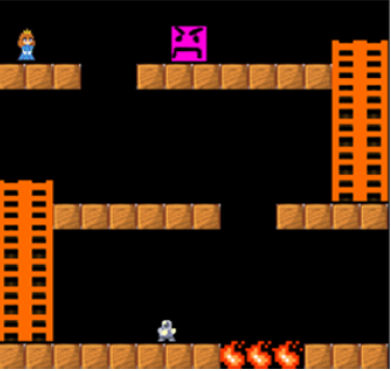
\includegraphics[width=\linewidth]{Figures/Example1a.png}
    \caption{Original State.}
  \end{subfigure}
  \begin{subfigure}[b]{0.45\linewidth}
    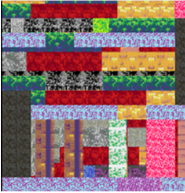
\includegraphics[width=\linewidth]{Figures/Example1b.png}
    \caption{Modified Game.}
  \end{subfigure}
  \caption{(a) A simple platformer game. (b) The same game modified by re-rendering the textures. Despite the two games being structurally the same, human players took twice as long to finish the second game as the first one. \cite{Dubey2018HumanPriors}}
  \label{fig:example}
\end{figure}

This paper will present a series of studies on a specially-designed game environment, The full game (unlike the first example) is going to be designed to be sufficiently complex for humans, taking into account the abovementioned factors, to easily measure the difficulty factors.

We are going to take the human as a logical being and test it on several settings where we vary such difficulty factors. It should be noted here that our aim is not to understand how humans learn a particular task (game) or how are they going to handle that task, but rather understand the entire process and to assess which types of task attributes affect human performance and how.

In addition to prior knowledge about objects, humans also bring in rich prior knowledge about intuitive physics and strong motor control priors when they approach a new task. Here, we have taken some initial steps to explore the importance of such priors in the context of human gameplay.

It is our contention in this paper that games that seem very different at first glance may be very similar at a more abstract level and beyond their immediate facade, games can be defined in terms of a number of factors, and furthermore it is these factors that define the complexity of a game and the best strategy to play it well.

-The factors mentioned above arise from the following questions:

-The number of players. Is the game played by a single player or multiple players, or does a single-player play with/against computer-controlled enemy units?

-Stochasticity. Is the outcome of the game determined only by the player?

-Time granularity. Is the game turn-based or real-time?

-Observability. Is the game partially observable or does the player have perfect information?

-Action space size. The number of actions the player can take.


In our case, we will analyze humans as the game-learners and consider games that can be played similarly to the ATARI 2600 games (Pac-Man, private eye, asteroids, etc...), where we can define and test the effect of such factors. Using average game scores, we will analyze the success of the task and how to perfect it. 
For instance, if the task is jumping on a vertically moving enemy, like in platforming game scores will depend on timing. If the jump is made at the right time, the score will be higher than if the jump is made out of time. In that way, we can assess the accuracy of the action in comparison with the skill being observed.

The results of Damien Anderson show that all tested AI agents are vulnerable to several kinds of deception, but those different agents have different weaknesses. This suggests that we can use deception to understand the capabilities of a game-playing algorithm, and game-playing algorithms to characterize the deception displayed by a game. If we use this logic with humans, we could ideally be able to discern other difficult factors for humans in games that may help us to create new difficulty paradigms. \cite{Anderson2018Deceptive}

At this point, we have used the term of difficulty in games without providing any definition of this word. We will not attempt to provide a general definition of difficulty covering a wide range of psychological aspects from emotional problems to intellectual and physical challenges. Instead, we consider the notion of difficulty in the sense used in game design, that is video games are built as combinations or sequences of predefined challenges. Thus, the study of the overall difficulty for a given video game involves studying the difficulty factors players experiment when overcoming a task.  \cite{Aponte2011DifVideoGames}

Dynamic Difficulty Adjustment: Rather than presenting every player with the same difficulty, some games tailor the difficulty presented to each player using Dynamic Difficulty Adjustment (DDA). DDA is a general term for techniques used to dynamically modify in-game difficulty during the course of gameplay as a means to tailor the experience more toward the player’s current level of play. This has been achieved in games through various techniques such as parameter tuning, modifying the level design, machine learning, the use of rating systems and player modeling. \cite{Sarkar2019TransDif}

In the current investigation, we will not focus on AI, but further research could to compare these factors with AIs and humans, and analyzing if these difficulty factors affect both subjects. We estimate the AIs will present a better performance, yet also problems with some logical tasks like in Montezuma revenge or private eye or many others (ATARI 2600 games), According to some research, a very popular setting for a general-purpose evaluation today is the collection of games or tasks under an interactive scenario, where agents can perceive and act and are rewarded when they succeed. Many different platforms have recently appeared for that. Some benchmarks that have become particularly popular in the past years are the Arcade Learning Environment (ALE) and General Video Game Artificial Intelligence (GVGAI). \cite{Bontrager2019Superstition, Anderson2018Deceptive, Plumed2018DualIn}
%\section{Objectives}
%\section{Structure of the Report}


\newpage